% DriftSense manuscript prepared for Human Technology.
% Compile with: xelatex main.tex; biber main; xelatex main.tex; xelatex main.tex
\documentclass[12pt,a4paper]{article}

\usepackage[top=3.8cm,bottom=3.7cm,left=2.54cm,right=2.54cm]{geometry}
\usepackage{fontspec}
\setmainfont{Times New Roman}
\newfontfamily\headingfont{Arial}
\usepackage{microtype}
\usepackage{setspace}
\singlespacing
\usepackage{graphicx}
\graphicspath{{figures/}}
\usepackage{booktabs}
\usepackage{tabularx}
\usepackage{array}
\usepackage{enumitem}
\usepackage{amsmath}
\usepackage{xcolor}
\usepackage{tikz}
\usetikzlibrary{arrows.meta,positioning,fit,calc,shapes.geometric}
\usepackage{caption}
\usepackage{subcaption}
\usepackage{titlesec}
\usepackage{fancyhdr}
\usepackage{etoolbox}
\usepackage[
  backend=biber,
  style=apa,
  sorting=nyt,
  sortcites=true,
  maxcitenames=99,
  mincitenames=99,
  maxbibnames=99,
  doi=true,
  url=false,
  isbn=false
]{biblatex}
\addbibresource{references.bib}
\newcommand{\citep}[1]{\parencite{#1}}
\usepackage{xurl}
\usepackage[hidelinks]{hyperref}

\definecolor{dsNavy}{HTML}{193A5A}
\definecolor{dsBlue}{HTML}{3E78B2}
\definecolor{dsGreen}{HTML}{16836E}
\definecolor{dsGold}{HTML}{D88918}
\definecolor{dsRed}{HTML}{C95852}
\definecolor{dsPaleBlue}{HTML}{EAF2FA}
\definecolor{dsPaleGreen}{HTML}{E6F3F0}
\definecolor{dsPaleGold}{HTML}{FFF4E2}
\definecolor{dsPaleRed}{HTML}{FBEDEC}
\definecolor{dsRule}{HTML}{AAB5BF}

\setlength{\parindent}{0.75cm}
\setlength{\parskip}{0pt}
\setlength{\emergencystretch}{4em}
\hyphenpenalty=10000
\exhyphenpenalty=10000
\setlist{nosep,leftmargin=1.1cm}
\setcounter{secnumdepth}{0}
\titleformat{\section}{\headingfont\bfseries\fontsize{12}{14}\selectfont\centering}{}{0pt}{\MakeUppercase}
\titleformat{\subsection}[block]{\headingfont\bfseries\fontsize{12}{14}\selectfont}{}{0pt}{}
\titleformat{\subsubsection}[block]{\headingfont\fontsize{12}{14}\selectfont}{}{0pt}{}
\titlespacing*{\section}{0pt}{18pt}{8pt}
\titlespacing*{\subsection}{0pt}{12pt}{4pt}
\titlespacing*{\subsubsection}{0.75cm}{10pt}{3pt}
\DeclareCaptionFont{arialnine}{\headingfont\fontsize{9}{11}\selectfont}
\captionsetup{font=arialnine,labelfont=bf,labelsep=period,justification=centering,singlelinecheck=false,skip=5pt}
\captionsetup[subfigure]{font=arialnine,labelfont=bf,labelsep=period,justification=centering}
\renewcommand{\arraystretch}{1.16}
\newcolumntype{Y}{>{\raggedright\arraybackslash}X}
\AtBeginEnvironment{table}{\headingfont\fontsize{9}{11}\selectfont}
\AtBeginEnvironment{tikzpicture}{\headingfont\fontsize{8.5}{10}\selectfont}

\pagestyle{fancy}
\fancyhf{}
\fancyfoot[C]{\thepage}
\renewcommand{\headrulewidth}{0pt}
\fancypagestyle{plain}{\fancyhf{}\fancyfoot[C]{\thepage}\renewcommand{\headrulewidth}{0pt}}

\begin{document}
\thispagestyle{plain}

\begin{center}
{\headingfont\bfseries\fontsize{15}{18}\selectfont
DRIFTSENSE: PRIVACY-MINIMIZED BROWSER TASK-DRIFT SENSING WITH A TANGIBLE REFLECTIVE INTERFACE\par}
\vspace{14pt}
\begin{minipage}[t]{0.31\textwidth}
\centering\headingfont
{\bfseries\fontsize{11}{13}\selectfont Sabbir Hossain\textsuperscript{*}\par}
{\fontsize{8.8}{10.5}\selectfont \phantom{Associate Professor}\par}
{\fontsize{9}{10.5}\selectfont Department of Computer Science\par
American International\par
University-Bangladesh\par
Dhaka, Bangladesh\par}
\vspace{2pt}
{\fontsize{8.3}{10}\selectfont \href{mailto:26-94030-1@student.aiub.edu}{26-94030-1@student.aiub.edu}\par}
\end{minipage}\hfill
\begin{minipage}[t]{0.31\textwidth}
\centering\headingfont
{\bfseries\fontsize{11}{13}\selectfont Pritam Banik\par}
{\fontsize{8.8}{10.5}\selectfont \phantom{Associate Professor}\par}
{\fontsize{9}{10.5}\selectfont Department of Computer Science\par
American International\par
University-Bangladesh\par
Dhaka, Bangladesh\par}
\vspace{2pt}
{\fontsize{8.3}{10}\selectfont \href{mailto:25-93822-2@student.aiub.edu}{25-93822-2@student.aiub.edu}\par}
\end{minipage}\hfill
\begin{minipage}[t]{0.31\textwidth}
\centering\headingfont
{\bfseries\fontsize{11}{13}\selectfont Abdus Salam\par}
{\fontsize{8.8}{10.5}\selectfont Associate Professor\par}
{\fontsize{9}{10.5}\selectfont Department of Computer Science\par
American International\par
University-Bangladesh\par
Dhaka, Bangladesh\par}
\vspace{2pt}
{\fontsize{8.3}{10}\selectfont \href{mailto:abdus.salam@aiub.edu}{abdus.salam@aiub.edu}\par}
\end{minipage}
\vspace{5pt}

{\headingfont\fontsize{8.8}{10.5}\selectfont \textsuperscript{*}Corresponding author: Sabbir Hossain\par}
\end{center}

\section*{Abstract}
\noindent Browser sites are mixed-use environments, so neither hostname nor elapsed time determines whether activity serves a user's current task. DriftSense is a local-first browser system with a tangible interface for participant-reported task drift. In Phase 1, 19 participants contributed 665 explicitly initiated sessions containing structured task context, content-free activity counts, and post-session alignment reports. A compact logistic model showed strong completed-session discrimination on a chronological holdout (ROC--AUC = .938; F1 = .870). Phase 2 applied the model through successive five-minute windows for sessions up to 20 minutes and ten-minute windows for longer sessions. Scores above threshold activated an ESP32 interface with a countdown display, brief buzzer cue, and three physical controls. Interviews with 12 participants indicated high usability, privacy comfort, usefulness, and low annoyance, while identifying mistimed cues. These findings support privacy-minimized reflective assistance while leaving early-window accuracy and causal behavioral effects for controlled evaluation.

\vspace{6pt}
\noindent\textbf{Keywords:} digital wellbeing; task alignment; browser activity; privacy-minimized sensing; tangible interaction; reflective intervention

\section{Introduction}

The same browser site can support sharply different goals. A video platform may host a tutorial, a social platform may contain a project discussion, and a search result may be either necessary background or the beginning of an unplanned detour. Treating a domain as inherently useful or distracting ignores this ambiguity. Fixed timers have a related weakness: they know how long a session has lasted but not whether the activity still serves the task that motivated it. DriftSense starts from a different premise. The participant declares the task, lightweight browser signals describe how the session unfolds, and the participant's later self-report defines whether drift occurred.

Digital self-control tools have commonly used blocking, time limits, reminders, monitoring, or interface restriction \citep{lyngs2019selfcontrol,biedermann2021digital,roffarello2023digital}. Reviews warn that screen time alone does not describe whether use was meaningful or whether an intervention respected the user's goal \citep{almoallim2022functionalities,rahmillah2023apps}. Purpose Mode preserves access while reducing selected attention-capturing elements \citep{lee2025purpose}; \textit{one sec} inserts a short pause before application entry \citep{gruning2023onesec}; and StayFocused asks reflective questions around attempted focus-session exits \citep{li2024stayfocused}. These systems motivate cues that are noticeable and optional rather than blocking.

We define \emph{browser task drift} as a participant's report that their browser activity moved away from the structured task declared at session start. This construct is not inferred attention, objective productivity, or a clinical condition. A switch away from an approved task site is not automatically drift, because a task may require supporting material elsewhere. Similarly, scrolling, idling, typing, or video playback can be either task-relevant or unrelated. DriftSense therefore treats activity signals as predictive evidence and preserves the participant's answer as the outcome.

The completed work followed two phases. Phase 1 was the data-collection and model-development phase: 19 participants contributed 665 sessions, of which 634 contained explicit binary alignment labels. Phase 2 was the main interactive product phase: the frozen local model evaluated successive activity windows and, when its score reached the threshold, activated a tangible ESP32 interface. The interface combined a 16x2 character display, an audible cue, and three physical buttons for session setup, completion, and reflection. Twelve participants then completed a structured post-study interview covering both phases.

The paper uses six terms consistently. A \emph{task session} is a period the participant explicitly starts for a declared task; opening a site alone does not start one. A \emph{participant-approved task site} is a hostname selected for planned work, not a site classified as productive. \emph{Task drift} is an explicit post-session report that activity moved away from the declared task. A \emph{content-free activity signal} is a count, duration, or state---such as clicks, active time, or tab focus---that stores no page text or typed characters. A \emph{rolling window} is the immediately preceding five- or ten-minute interval evaluated at a checkpoint. The \emph{tangible reflective interface} is the physical LCD, buzzer, and buttons that present session state and let the participant respond without blocking the browser.

This paper asks three questions:

\begin{enumerate}[label=\textit{RQ\arabic*:},font=\itshape]
\item How can a browser system represent participant-declared task alignment using privacy-minimized, content-free signals without treating time or hostnames as ground truth?
\item How well does the Phase 1 model distinguish later participant-reported task drift on a chronological completed-session holdout?
\item How did participants describe the usability, privacy, timing, usefulness, interruption, and annoyance of the Phase 2 tangible interface?
\end{enumerate}

The contribution is an end-to-end HCI system rather than a generic activity tracker. It comprises a participant-grounded task-drift construct, a local sensing and labeling workflow, a compact model and duration-dependent rolling policy, a tangible reflective interface, and empirical evidence from both session records and post-study interviews. Figure~\ref{fig:overview} summarizes the relationship between the two phases and the distinct evidence each produced.

\begin{figure}[htbp]
\centering
\resizebox{0.99\textwidth}{!}{%
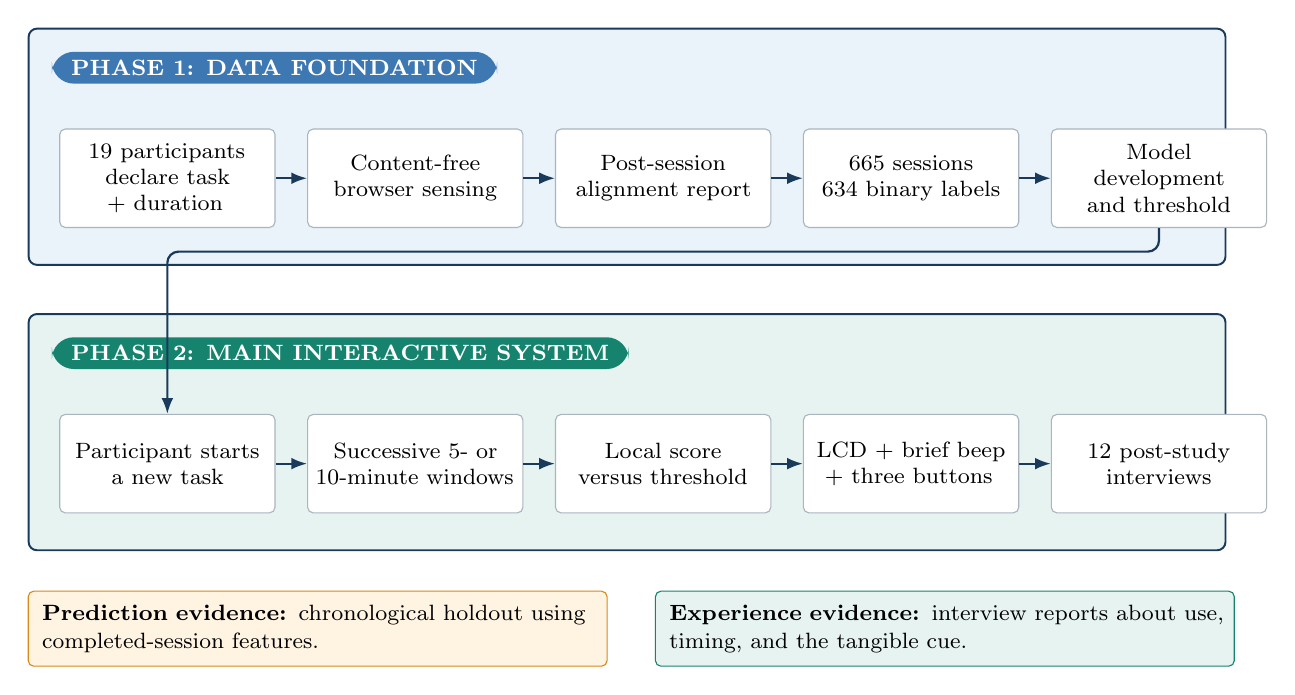
\begin{tikzpicture}[
  node distance=4.5mm,
  phase/.style={rounded corners=3pt,draw=dsNavy,line width=.7pt,minimum width=15.2cm,minimum height=3.0cm,inner sep=6pt},
  stagebox/.style={rounded corners=2pt,draw=dsRule,fill=white,align=center,text width=2.5cm,minimum height=1.25cm,font=\headingfont\fontsize{8.2}{9.5}\selectfont},
  arrow/.style={-{Latex[length=2mm]},line width=.8pt,draw=dsNavy},
  tag/.style={rounded corners=8pt,inner xsep=7pt,inner ysep=3pt,font=\headingfont\bfseries\fontsize{8.5}{10}\selectfont}
]
\node[phase,fill=dsPaleBlue] (p1) {};
\node[tag,fill=dsBlue,text=white,anchor=north west] at ($(p1.north west)+(3mm,-3mm)$) {PHASE 1: DATA FOUNDATION};
\node[stagebox,anchor=west] (s1) at ($(p1.west)+(4mm,-4mm)$) {19 participants\\declare task + duration};
\node[stagebox,right=4mm of s1] (s2) {Content-free\\browser sensing};
\node[stagebox,right=4mm of s2] (s3) {Post-session\\alignment report};
\node[stagebox,right=4mm of s3] (s4) {665 sessions\\634 binary labels};
\node[stagebox,right=4mm of s4] (s5) {Model\\development\\and threshold};
\draw[arrow] (s1)--(s2); \draw[arrow] (s2)--(s3); \draw[arrow] (s3)--(s4); \draw[arrow] (s4)--(s5);

\node[phase,fill=dsPaleGreen,below=6mm of p1] (p2) {};
\node[tag,fill=dsGreen,text=white,anchor=north west] at ($(p2.north west)+(3mm,-3mm)$) {PHASE 2: MAIN INTERACTIVE SYSTEM};
\node[stagebox,anchor=west] (t1) at ($(p2.west)+(4mm,-4mm)$) {Participant starts\\a new task};
\node[stagebox,right=4mm of t1] (t2) {Successive 5- or\\10-minute windows};
\node[stagebox,right=4mm of t2] (t3) {Local score\\versus threshold};
\node[stagebox,right=4mm of t3] (t4) {LCD + brief beep\\+ three buttons};
\node[stagebox,right=4mm of t4] (t5) {12 post-study\\interviews};
\draw[arrow] (t1)--(t2); \draw[arrow] (t2)--(t3); \draw[arrow] (t3)--(t4); \draw[arrow] (t4)--(t5);
\draw[arrow,rounded corners] (s5.south) -- ++(0,-3mm) -| (t1.north);

\node[rounded corners=2pt,draw=dsGold,fill=dsPaleGold,align=left,text width=7cm,inner sep=5pt,anchor=north west,font=\fontsize{8.5}{10}\selectfont] (e1) at ($(p2.south west)+(0,-5mm)$) {\textbf{Prediction evidence:} chronological holdout using completed-session features.};
\node[rounded corners=2pt,draw=dsGreen,fill=dsPaleGreen,align=left,text width=7cm,inner sep=5pt,right=6mm of e1,font=\fontsize{8.5}{10}\selectfont] (e2) {\textbf{Experience evidence:} interview reports about use, timing, and the tangible cue.};
\end{tikzpicture}
}
\caption{DriftSense's completed two-phase workflow. Phase 1 produced the participant-labeled data and model. Phase 2 operationalized the model through duration-dependent checks and a tangible reflective interface. The two evidence streams answer different questions and are not combined into a causal effectiveness claim.}
\label{fig:overview}
\end{figure}

\section{Related Work}

\subsection{Digital Self-Control and Preserving Utility}

Digital self-control tools span dashboards, timers, application limits, blocking, friction, reminders, and interface changes \citep{lyngs2019selfcontrol,roffarello2023digital}. Recent reviews find mixed evidence across short, varied studies and call for designs that go beyond screen-time reduction \citep{biedermann2021digital,plackett2023socialmedia,almoallim2022functionalities,almansoori2023designing}. Digital wellbeing is better understood as a changing balance between technology's benefits and costs than as the absence of use \citep{vandenabeele2020dynamic}. Less use may mean successful self-regulation or unfinished work; more use may mean drift or necessary effort.

Interface design can also shape user agency \citep{monge2023acdp,cecchinato2019agenda}. Controlled studies of social-media interfaces show that the same restriction can help in one context and create friction in another \citep{lyngs2020facebook}. Purpose Mode lets users hide feeds, constrain continuous content, or simplify layouts \citep{lee2025purpose}. Earlier work similarly found that people judge smartphone use partly through purpose and autonomy rather than duration alone \citep{lukoff2018meaningful}. These findings explain why DriftSense does not classify an entire site as undesirable or block access when a cue appears.

\subsection{Intention, Friction, and Reflection}

Interventions can interrupt automatic action without imposing a prohibition. \textit{one sec} couples a short delay with an explicit choice before entry to a selected application \citep{gruning2023onesec}. MindPhone asks about intention at phone unlock \citep{terzimehic2022mindphone}; StayFocused asks reflective questions around a focus-session exit \citep{li2024stayfocused}; and InteractOut adds weak resistance to common gestures \citep{lu2024interactout}. A large review of goal-oriented HCI interventions further shows that the way a goal is represented and supported matters to behavior-change outcomes \citep{zhu2025goals}.

PauseNow frames digital wellbeing as alignment between intention and behavior rather than simple screen-time reduction \citep{zhao2024pausenow}. WellScreen compares expected and observed use to support reflection \citep{bhat2026wellscreen}. Regret also depends on both intention and activity \citep{cho2021reflect}. DriftSense therefore asks for the task before use and alignment after use; its cue invites reconsideration without claiming to know the participant's internal state.

Some recent systems use richer semantic inputs to infer mental states or examine regretted use \citep{wu2024mindshift,guo2025regret}. These approaches can support detailed interpretation, but they also require more sensitive content than DriftSense stores. DriftSense instead limits its model to structured task context and aggregate, content-free activity.

\subsection{Tangible and Audible Interaction}

A tangible user interface gives digital state a physical form that can be seen or manipulated \citep{ishii1997tangible}. Recent reviews describe tangible systems as especially useful when controls should remain visible, direct, and separate from a crowded screen, while also stressing the need for usability evaluation before stronger outcome claims \citep{bertolo2025tangible}. Sound is similarly noticeable outside the visual foreground, but it can interrupt or create social discomfort. Studies of notification muting show that removing sound does not automatically reduce checking or improve wellbeing \citep{liao2022sound,dekker2025buzz}. DriftSense therefore uses a short, time-limited beep paired with a display and physical controls, and the interviews explicitly measure interruption and annoyance.

\subsection{Behavioral Sensing, Personal Context, and Privacy}

Behavioral sensing can support timely assistance, but richer sensing also increases disclosure risk. Digital-wellbeing scholarship therefore calls for attention to agency, context, and the consequences of measurement \citep{burr2020ethics,buchi2021digital}. Studies across devices also show that wellbeing practices and constraints do not stop at one screen \citep{roffarello2021multidevice}. DriftSense therefore reports its known-participant holdout without claiming unseen-user performance.

DriftSense minimizes inputs rather than reconstructing page meaning. It records structured task type, timing, interaction counts without their values, focus state, idle and active time, aggregate away time without destination identity, and accessible video-playback state. It excludes page text, titles, URL paths and queries, messages, screenshots, key values, and outside-set destination identities. This retains useful session patterns while reducing exposure of what the participant viewed or typed.

\subsection{Research Gap}

Existing systems provide interface modification, pre-access friction, reflective prompts, intention questions, or post-use awareness. DriftSense links these elements at browser-session level: the participant starts a task, content-free activity is summarized locally, the post-session answer supplies the label, the model evaluates five- or ten-minute windows, and a physical device delivers a brief cue outside the browser. Table~\ref{tab:related} compares the closest systems.

\begin{table}[htbp]
\centering
\caption{Closest Systems and the Design Gap Addressed by DriftSense.}
\label{tab:related}
\small
\begin{tabularx}{\textwidth}{@{}p{2.7cm}YYYY@{}}
\toprule
System & Intervention moment & Role of intention & Evidence & Difference from DriftSense \\
\midrule
Purpose Mode \citep{lee2025purpose} & During social-media use & Goal alignment measured in repeated assessments & Two-week field deployment & Modifies interface features; no session classifier or tangible cue \\
\textit{one sec} \citep{gruning2023onesec} & Before application access & Opening reason supports deliberation & Observational deployment and online experiment & Fixed friction before entry rather than model-timed reflection \\
StayFocused \citep{li2024stayfocused} & On attempted exit or session completion & Focus goal entered at session start & Three-condition field study & Triggered by interaction state rather than activity-based risk \\
PauseNow \citep{zhao2024pausenow} & Proposed recognition and nudging & Original intention is central & Conceptual framework & No deployed prediction and outcome evaluation \\
WellScreen \citep{bhat2026wellscreen} & Daily post-use reflection & Estimated versus observed use & Two-week mixed-methods probe & Retrospective daily reflection rather than within-session cueing \\
\textbf{DriftSense} & Successive 5- or 10-minute windows & Task declared before use; alignment answered afterward & 665 sessions and 12 interviews & Local content-free model linked to an ESP32 reflective interface \\
\bottomrule
\end{tabularx}
\end{table}

\section{DriftSense Concept and Design}

\subsection{Task Drift as a Participant-Grounded Construct}

DriftSense separates context, predictors, and outcomes. The participant-approved hostname and structured task type provide context. Aggregate activity provides predictors. Only the explicit post-session alignment response supplies the binary outcome. This separation prevents a common category error: treating a behavioral trace as if it were proof of what the behavior meant.

At task start, a participant chooses one of six structured task types: writing or creating, coding or problem solving, reading or research, learning or tutorial, communication or coordination, or another planned task. The participant also selects an intended duration. The duration configures the session and rolling schedule but does not automatically end the task or label its outcome. The task may continue across multiple approved sites, and temporary activity away from the approved set remains an aggregate duration rather than a record of destination identity.

At the real session boundary, DriftSense asks whether the session remained aligned with the task the participant started. An explicit aligned response is coded 0 and an explicit moved-away response is coded 1. A not-sure response, a missing answer, or an action without an alignment answer remains unlabeled. Continue, save, dismiss, stop, and reminder actions are not substituted for the construct.

\subsection{Design Requirements}

Six requirements shaped the implementation:

\begin{enumerate}
\item \textbf{Explicit initiation.} A hostname opening is not sufficient evidence of a task; the participant starts the session and declares a structured task type.
\item \textbf{Participant-defined alignment.} Time and site are inputs or baselines, never ground-truth labels.
\item \textbf{Content minimization.} The system uses counts, durations, and states without collecting page content or key values.
\item \textbf{Local operation.} Session records, model parameters, and exports remain on the participant's device unless the participant deliberately exports them.
\item \textbf{User-controlled support.} A cue is brief and nonblocking, displays no probability, and permits the participant to continue intentionally.
\item \textbf{Auditable state.} Session, checkpoint, model, cue, response, and suppression states are represented explicitly so that prediction and outcome measurement remain separable.
\end{enumerate}

\subsection{Browser and Tangible Components}

The browser component is a Chrome Manifest V3 extension implemented with React and TypeScript. Its background service worker manages a single active task session, local storage, activity aggregation, pending reflections, checkpoint evaluation, and exports. Content scripts count clicks, scroll events, and keyboard activity without storing targets or characters. Focus, idle, active, away, tab-switch, and accessible video-playback durations are accumulated in ten-second windows.

The extension includes onboarding, participant-approved task-site configuration, a task-start popup, local dashboards, a privacy and export view, and an ESP32 controller page. Figure~\ref{fig:interfaces} shows the two views that most directly explain the interaction sequence. The popup makes task declaration and intended duration visible before data collection. The device controller mirrors the physical controls and the LCD state, making the hardware behavior inspectable even though the ESP32 remains the immediate tangible interface. The privacy boundary is documented separately in Figure~\ref{fig:privacy}.

\begin{figure}[htbp]
\centering
\begin{subfigure}[t]{0.29\textwidth}
\centering
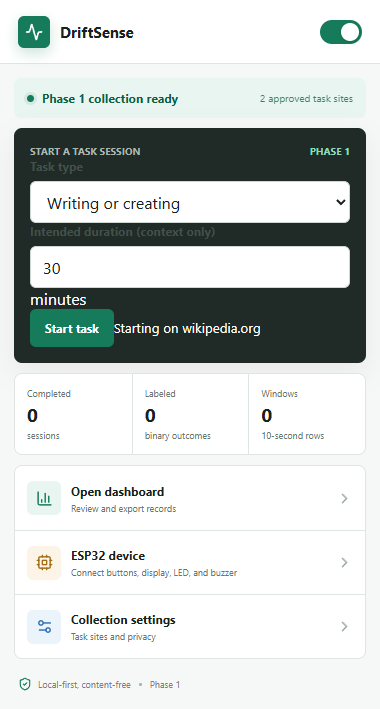
\includegraphics[width=\linewidth]{driftsense-popup.png}
\caption{Task-start popup.}
\end{subfigure}\hfill
\begin{subfigure}[t]{0.68\textwidth}
\centering
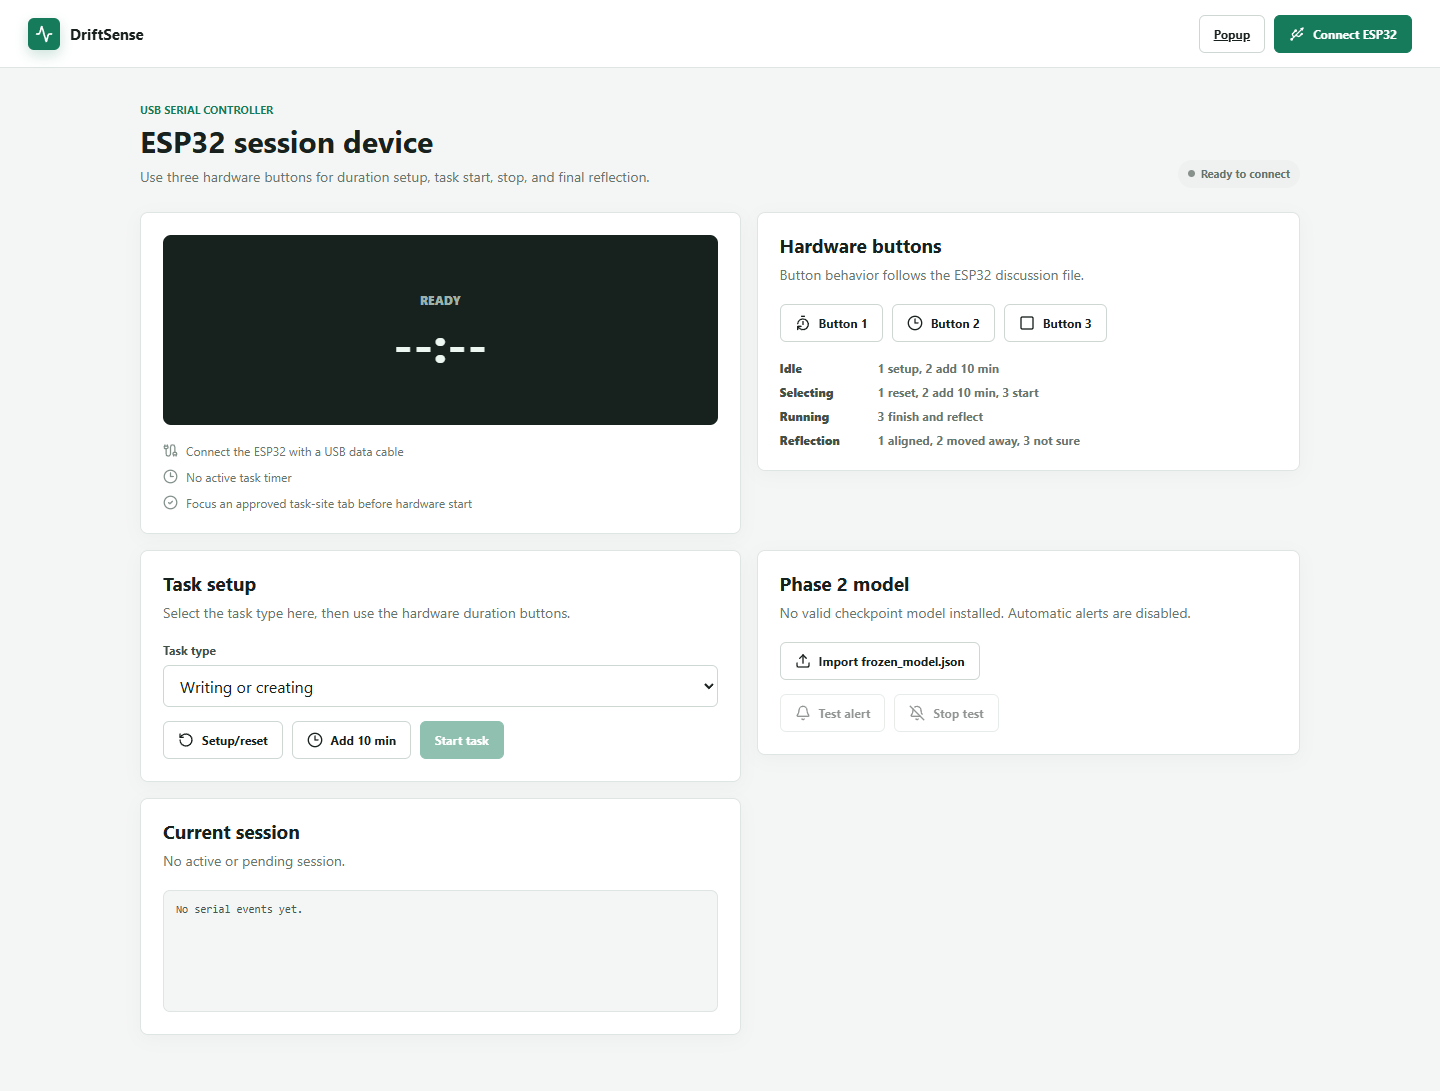
\includegraphics[width=\linewidth,trim=140 541 140 65,clip]{driftsense-device-page.png}
\caption{ESP32 controller and button map.}
\end{subfigure}

\caption{Implemented DriftSense browser interfaces. The task-start popup makes the declared task and duration explicit, while the cropped controller view shows the browser-side liquid-crystal display (LCD) representation and state-dependent mapping of the three physical buttons. ESP32 denotes the microcontroller platform.}
\label{fig:interfaces}
\end{figure}

The ESP32 device uses a 16x2 I2C character display, three pull-up buttons, and an active buzzer. The display maintains the selected duration and countdown. Button meanings change with a small number of visible states: setup, selection, running, and reflection. During setup, the buttons reset or add duration and start the task. During a running session, the third button finishes the task and requests reflection. During reflection, buttons 1, 2, and 3 record aligned, moved away, and not sure, respectively. The device and extension exchange short line-based commands over USB serial; the browser remains the source of truth for session and model state.

When a model score reaches the threshold, the device produces two short beeps every ten seconds for at most five cycles. Returning to an approved task site, completing the task, entering reflection, pressing stop, or reaching the automatic limit silences the buzzer. A two-second heartbeat lets the device detect connection loss; an unresolved alert is silenced after 15 seconds without a heartbeat. These rules keep the cue noticeable and time-limited.

\begin{figure}[htbp]
\centering
\resizebox{0.99\textwidth}{!}{%
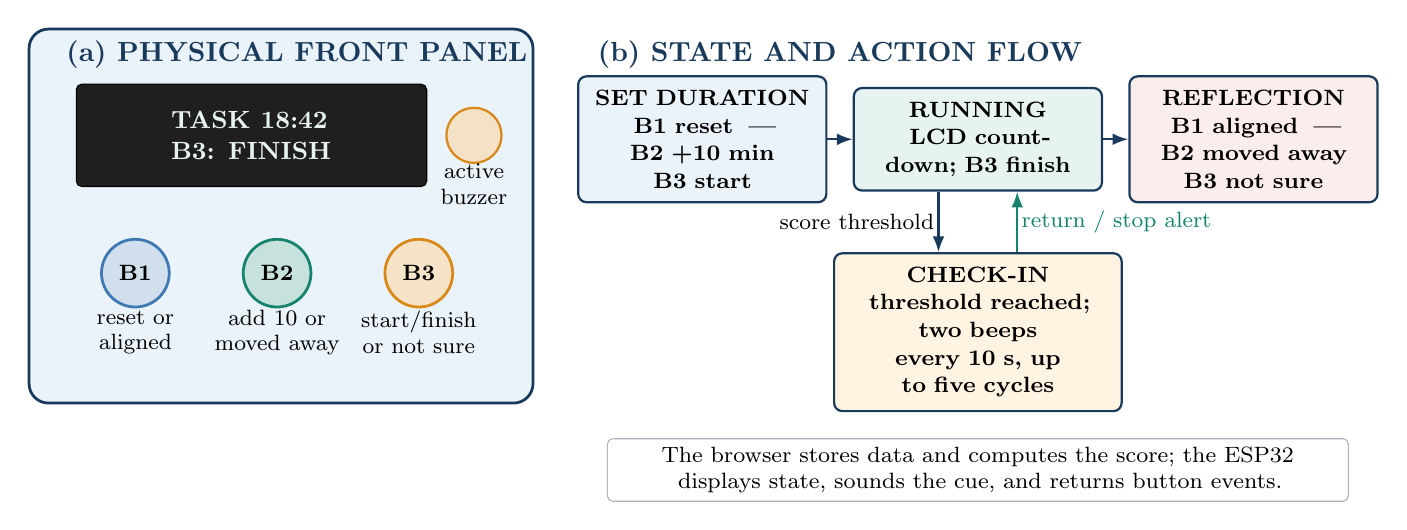
\begin{tikzpicture}[
 state/.style={rounded corners=3pt,draw=dsNavy,line width=.8pt,align=center,text width=3.15cm,minimum height=1.15cm,inner sep=5pt,font=\fontsize{8.5}{10}\selectfont},
 arrow/.style={-{Latex[length=2mm]},line width=.8pt,draw=dsNavy},
 note/.style={font=\headingfont\fontsize{8}{9.2}\selectfont,align=center},
 edgelabel/.style={font=\headingfont\fontsize{8}{9.2}\selectfont,align=center,fill=white,inner sep=1.2pt}
]
\draw[rounded corners=7pt,draw=dsNavy,line width=1pt,fill=dsPaleBlue] (.2,-2.0) rectangle (6.6,2.75);
\node[anchor=west,font=\headingfont\bfseries\fontsize{10}{12}\selectfont,text=dsNavy] at (.55,2.43) {(a) PHYSICAL FRONT PANEL};
\draw[rounded corners=2pt,fill=black!88,draw=black] (.8,.75) rectangle (5.25,2.05);
\node[text=dsPaleGreen,font=\headingfont\bfseries\fontsize{9}{11}\selectfont,align=left] at (3.02,1.40) {TASK 18:42\\B3: FINISH};
\draw[fill=dsGold!25,draw=dsGold,line width=.8pt] (5.85,1.40) circle (.35);
\node[note] at (5.85,.78) {active\\buzzer};
\foreach \x/\button/\colour in {1.55/B1/dsBlue,3.35/B2/dsGreen,5.15/B3/dsGold}{
  \draw[fill=\colour!24,draw=\colour,line width=1pt] (\x,-.35) circle (.43);
  \node[font=\headingfont\bfseries\fontsize{8.5}{10}\selectfont] at (\x,-.35) {\button};
}
\node[note] at (1.55,-1.10) {reset or\\aligned};
\node[note] at (3.35,-1.10) {add 10 or\\moved away};
\node[note] at (5.15,-1.10) {start/finish\\or not sure};

\node[anchor=west,font=\headingfont\bfseries\fontsize{10}{12}\selectfont,text=dsNavy] at (7.3,2.43) {(b) STATE AND ACTION FLOW};
\node[state,fill=dsPaleBlue,text width=2.8cm] (select) at (8.75,1.35) {\headingfont\bfseries SET DURATION\\B1 reset \;|\; B2 +10 min\\B3 start};
\node[state,fill=dsPaleGreen,text width=2.8cm] (running) at (12.25,1.35) {\headingfont\bfseries RUNNING\\LCD countdown; B3 finish};
\node[state,fill=dsPaleRed,text width=2.8cm] (reflect) at (15.75,1.35) {\headingfont\bfseries REFLECTION\\B1 aligned \;|\; B2 moved away\\B3 not sure};
\node[state,fill=dsPaleGold,text width=3.3cm] (cue) at (12.25,-1.10) {\headingfont\bfseries CHECK-IN\\threshold reached; two beeps\\every 10 s, up to five cycles};
\draw[arrow] (select.east)--(running.west);
\draw[arrow] (running.east)--(reflect.west);
\draw[arrow] ([xshift=-5mm]running.south)--node[left,edgelabel]{score threshold}([xshift=-5mm]cue.north);
\draw[arrow,draw=dsGreen] ([xshift=5mm]cue.north)--node[right,edgelabel,text=dsGreen]{return / stop alert}([xshift=5mm]running.south);
\node[rounded corners=2pt,draw=dsRule,fill=white,text width=9.2cm,align=center,inner sep=3pt,font=\fontsize{8.2}{9.5}\selectfont] at (12.25,-2.85) {The browser stores data and computes the score; the ESP32 displays state, sounds the cue, and returns button events.};
\end{tikzpicture}
}
\caption{Tangible interface and state-dependent controls. Panel (a) shows the physical liquid-crystal display (LCD), buzzer, and three buttons. Panel (b) shows how the same controls support duration selection, a running task, a model-triggered check-in, and the final alignment response. B1--B3 denote buttons 1--3.}
\label{fig:hardware}
\end{figure}

\subsection{Privacy Boundary}

Privacy is an architectural constraint rather than only a policy statement. Figure~\ref{fig:privacy} groups stored data by purpose and contrasts them with excluded content. Approved hostnames identify only the sites a participant selected for planned tasks. Activity outside that set is summarized as away time without destination identity. The model receives numeric summaries and a structured task category, not page semantics. Participants can inspect, export, or delete their local records.

\begin{figure}[htbp]
\centering
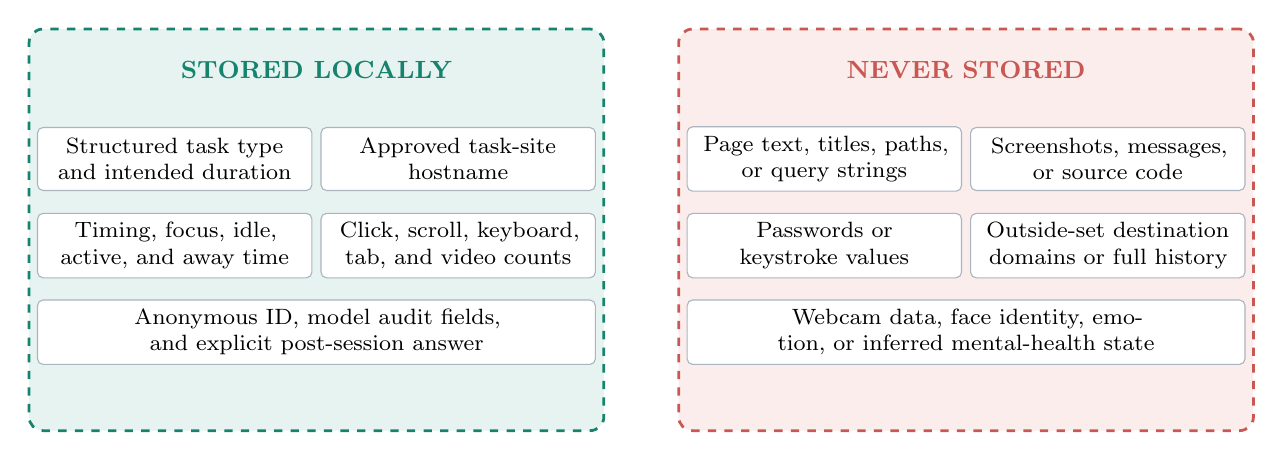
\begin{tikzpicture}[
 item/.style={rounded corners=2pt,draw=dsRule,fill=white,text width=3.25cm,minimum height=.8cm,align=center,font=\fontsize{8.3}{9.5}\selectfont},
 head/.style={font=\headingfont\bfseries\fontsize{9.5}{11}\selectfont},
 boundary/.style={rounded corners=5pt,dashed,line width=1pt,inner sep=6pt}
]
\node[boundary,draw=dsGreen,fill=dsPaleGreen,minimum width=7.3cm,minimum height=5.1cm] (stored) at (0,0) {};
\node[head,text=dsGreen,anchor=north] at ($(stored.north)+(0,-3mm)$) {STORED LOCALLY};
\node[item] at (-1.8,.9) {Structured task type\\and intended duration};
\node[item] at (1.8,.9) {Approved task-site\\hostname};
\node[item] at (-1.8,-.2) {Timing, focus, idle,\\active, and away time};
\node[item] at (1.8,-.2) {Click, scroll, keyboard,\\tab, and video counts};
\node[item,text width=6.85cm] at (0,-1.3) {Anonymous ID, model audit fields, and explicit post-session answer};

\node[boundary,draw=dsRed,fill=dsPaleRed,minimum width=7.3cm,minimum height=5.1cm] (excluded) at (8.25,0) {};
\node[head,text=dsRed,anchor=north] at ($(excluded.north)+(0,-3mm)$) {NEVER STORED};
\node[item] at (6.45,.9) {Page text, titles, paths,\\or query strings};
\node[item] at (10.05,.9) {Screenshots, messages,\\or source code};
\node[item] at (6.45,-.2) {Passwords or\\keystroke values};
\node[item] at (10.05,-.2) {Outside-set destination\\domains or full history};
\node[item,text width=6.85cm] at (8.25,-1.3) {Webcam data, face identity, emotion, or inferred mental-health state};
\end{tikzpicture}
\caption{DriftSense privacy boundary. The local record contains only structured task context, aggregate behavior, and explicit participant responses. It excludes page semantics and identifiable content. ID denotes anonymous participant identifier.}
\label{fig:privacy}
\end{figure}

\section{Methods}

\subsection{Study Structure and Evidence Sources}

The study used a sequential two-phase design. Phase 1 collected task-session records without a model-assisted mid-session cue. After the data were merged, checked, and used for model development, Phase 2 deployed the tangible system with duration-dependent model evaluation. The same task-alignment construct linked the phases, but the evidence served different purposes. Phase 1 supported model development and retrospective discrimination. Phase 2 interviews supported descriptive evaluation of usability and perceived cue experience. The phase order was fixed, so differences in preference or recollection are not randomized causal estimates.

Four evidence sources support the paper. The literature archive contains the works used to derive the design requirements and research gap. The extension, firmware, model artifacts, and automated tests establish implemented behavior. The merged session file provides Phase 1 activity and alignment records. The interview workbook provides anonymous structured and open responses from 12 participants after Phase 2.

\subsection{Phase 1 Data Collection}

Nineteen participants installed the extension and explicitly started browser task sessions. At each start they selected a structured task type and intended duration. During the task, the extension aggregated content-free interaction and state measures into local ten-second windows. At the session boundary it requested the participant's alignment answer and retained unresolved questions as pending reflections rather than silently assigning a label.

The participant exports were merged into \texttt{driftsense\_merged.csv}. The file contains 665 sessions and 18 documented fields. Participants contributed between 31 and 39 sessions (median = 35). Intended durations were 10, 15, 20, 30, 45, 60, or 90 minutes. Observed durations ranged from 1.6 to 120.0 minutes (median = 24.3; mean = 31.5). Learning or tutorial sessions were most common (199), followed by communication or coordination (129), reading or research (122), coding or problem solving (93), writing or creating (91), and other planned tasks (31).

Of the 665 records, 634 had usable binary outcomes: 358 aligned and 276 moved away, yielding a drift prevalence of 43.5\%. Thirty-one not-sure or missing outcomes were excluded from binary modeling. A consistency audit identified 20 rows in which the stored numeric label disagreed with the explicit post-session answer. The analysis derived the label from that explicit answer according to the study rule and left the source export unchanged. There were no duplicate session identifiers, no overlapping sessions within a participant, and all 665 rows satisfied exact active + idle + away time accounting.

\subsection{Model Development and Validation}

The modeling pipeline compared increasingly informative feature families: majority class, a prompt-all timer rule, intended duration, task site, task type, combined context, activity, context plus activity, context plus activity and elapsed-time features, and participant-calibrated context plus activity. Activity features included log-transformed event counts and durations, event rates per minute, and active, idle, away, and video shares. Participant identifiers organized the splits but were not included as model inputs.

Preprocessing was fit within training data. The development set contained participant-relative days 1--7 for all 19 participants (441 sessions). Candidate feature families and regularization values were compared using five repeats of participant-grouped five-fold validation. A chronological known-participant holdout contained 193 later sessions from 18 participants. The selection rule preferred the highest development ROC--AUC, choosing the simpler family when models were within .01 and then comparing Brier score. A decision threshold was selected on development predictions subject to a 35\% positive-decision cap and evaluated once on the chronological holdout.

The deployed Phase 2 package was a compact logistic model using structured task type, intended duration, task-site count, elapsed-to-intended-duration ratio, and active, idle, and away shares. It was serialized for matching browser-side inference. The stored threshold was .7363. The model's retrospective holdout results use completed-session activity proportions; they show discrimination in recorded sessions but do not prove accuracy for the earlier rolling windows used during Phase 2.

\subsection{Phase 2 Rolling Evaluation}

Phase 2 converted the model into a duration-sensitive interaction. Sessions with intended duration up to and including 20 minutes were checked every five minutes. Longer sessions were checked every ten minutes. Each checkpoint evaluated only the immediately preceding interval, as illustrated in Figure~\ref{fig:rolling}. Thus, minute 10 in a short session represents minutes 5--10, whereas minute 20 in a longer session represents minutes 10--20. The implementation continues this pattern for the configured duration; for example, a 50-minute session is checked at minutes 10, 20, 30, 40, and 50.

\begin{figure}[htbp]
\centering
\resizebox{0.99\textwidth}{!}{%
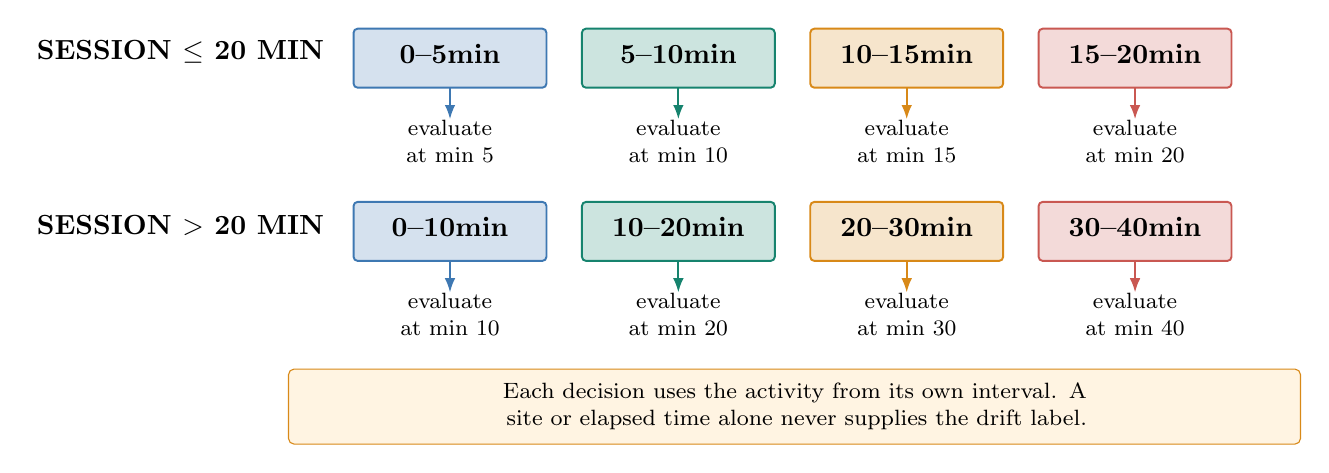
\begin{tikzpicture}[x=1cm,y=1cm,font=\fontsize{8.5}{10}\selectfont]
\node[anchor=east,font=\headingfont\bfseries] at (2.25,2.15) {SESSION $\leq$ 20 MIN};
\foreach \x/\a/\b/\c in {2.5/0/5/dsBlue,5.4/5/10/dsGreen,8.3/10/15/dsGold,11.2/15/20/dsRed}{
  \filldraw[fill=\c!22,draw=\c,line width=.7pt,rounded corners=1.5pt] (\x,1.7) rectangle ++(2.45,.75);
  \node[font=\headingfont\bfseries] at (\x+1.225,2.13) {\a--\b min};
  \draw[-{Latex[length=1.8mm]},draw=\c,line width=.7pt] (\x+1.225,1.7)--++(0,-.4);
  \node[align=center] at (\x+1.225,1.02) {evaluate\\at min \b};
}
\node[anchor=east,font=\headingfont\bfseries] at (2.25,-.05) {SESSION $>$ 20 MIN};
\foreach \x/\a/\b/\c in {2.5/0/10/dsBlue,5.4/10/20/dsGreen,8.3/20/30/dsGold,11.2/30/40/dsRed}{
  \filldraw[fill=\c!22,draw=\c,line width=.7pt,rounded corners=1.5pt] (\x,-.5) rectangle ++(2.45,.75);
  \node[font=\headingfont\bfseries] at (\x+1.225,-.07) {\a--\b min};
  \draw[-{Latex[length=1.8mm]},draw=\c,line width=.7pt] (\x+1.225,-.5)--++(0,-.4);
  \node[align=center] at (\x+1.225,-1.18) {evaluate\\at min \b};
}
\node[rounded corners=2pt,fill=dsPaleGold,draw=dsGold,text width=12.5cm,align=center,inner sep=5pt] at (8.1,-2.35) {Each decision uses the activity from its own interval. A site or elapsed time alone never supplies the drift label.};
\end{tikzpicture}
}
\caption{Implemented duration-dependent rolling schedule. Five-minute intervals are used for intended sessions up to 20 minutes; ten-minute intervals are used for longer sessions. The illustrated long-session sequence continues in ten-minute steps when the intended duration exceeds 40 minutes.}
\label{fig:rolling}
\end{figure}

At a checkpoint, a score below threshold produced no device cue. A score at or above threshold began one alert episode. The cue never displayed the score or stated that drift had occurred. The participant could return to the task, continue intentionally, or finish and answer the post-session question. The completed deployment delivered every cue whose score reached the threshold; it did not include a concurrent silent-control condition.

\subsection{Post-Study Interviews}

Twelve participants completed the interview workbook after using both phases. Six were aged 18--24, five were 25--34, and one was 35--44. Six identified their main role as student, two as knowledge worker, two as software professional, and two as both student and worker. Eleven remembered receiving the Phase 2 check-in and beep; one did not. Ratings specifically concerning cue timing and experience were therefore available for 11 participants, while general Phase 2 ratings and phase preference were available for all 12.

The workbook contains five Phase 1 and ten Phase 2 Likert statements on a five-point agreement scale. For positively worded items, ratings of 4 or 5 were favorable. For effort, interruption, and annoyance, ratings of 1 or 2 were favorable. We report valid $n$, median, interquartile range (IQR), and favorable count rather than treating the scale as a continuous measure. Open responses were grouped by useful effects, limitations, and requested refinements. Because independent coders were not documented, these groups summarize responses rather than claim a complete thematic analysis.

\section{Results}

\subsection{Phase 1 Dataset and Model Comparisons}

The Phase 1 dataset had broad coverage across the six task types and repeated observations for every participant. Its 634 labeled sessions provided 358 aligned and 276 moved-away outcomes. The chronological holdout retained later sessions from known participants rather than randomly mixing a participant's early and late records. This makes the result more demanding than a random session split, while still not constituting an unseen-participant test.

Context-only baselines performed modestly on the chronological holdout. Intended duration yielded ROC--AUC .551, task site .576, task type .620, and combined task context .631. Activity-only logistic regression increased ROC--AUC to .931. Adding context, elapsed-time features, or participant calibration produced ROC--AUC values from .932 to .936. The differences among these richer models were small, reinforcing the value of a compact model and cautioning against claims that any one context variable independently establishes alignment.

For the separately packaged Phase 2 model, the 193-session chronological holdout yielded ROC--AUC .938, accuracy .891, precision .959, recall .795, and F1 .870 at threshold .7363. The confusion matrix contained 102 true negatives, 3 false positives, 18 false negatives, and 70 true positives. Seventy-three of 193 sessions (37.8\%) crossed the threshold. Figure~\ref{fig:modelresults} presents the baseline progression and operational scorecard.

\begin{figure}[htbp]
\centering
\resizebox{0.99\textwidth}{!}{%
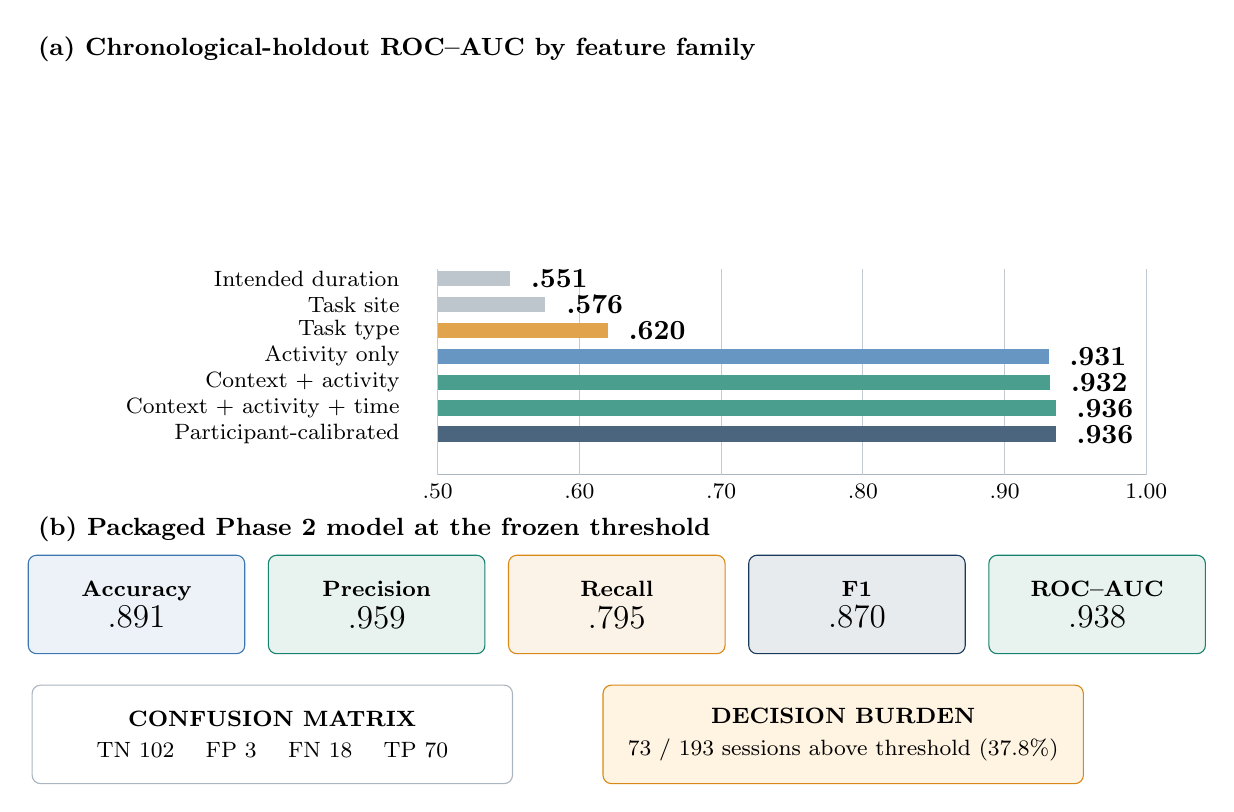
\begin{tikzpicture}[font=\fontsize{8.2}{9.5}\selectfont]
\node[anchor=west,font=\headingfont\bfseries\fontsize{9.5}{11}\selectfont] at (0,5.4) {(a) Chronological-holdout ROC--AUC by feature family};
\begin{scope}[xshift=5.2cm,x=18cm,y=.55cm]
  \draw[draw=dsRule] (0,0)--(.5,0);
  \foreach \x/\lab in {0/.50,.1/.60,.2/.70,.3/.80,.4/.90,.5/1.00}{\draw[draw=dsRule!70] (\x,0)--(\x,4.75);\node[below] at (\x,0){\lab};}
  \foreach \y/\name/\v/\score/\col in {4.35/Intended duration/.051/.551/dsRule,3.75/Task site/.076/.576/dsRule,3.15/Task type/.120/.620/dsGold,2.55/Activity only/.431/.931/dsBlue,1.95/Context + activity/.432/.932/dsGreen,1.35/Context + activity + time/.436/.936/dsGreen,.75/Participant-calibrated/.436/.936/dsNavy}{
    \node[anchor=east] at (-.02,\y+.18) {\name};
    \fill[\col!78] (0,\y) rectangle (\v,\y+.36);
    \node[anchor=west,font=\bfseries] at (\v+.008,\y+.18) {\score};
  }
\end{scope}

\node[anchor=west,font=\headingfont\bfseries\fontsize{9.5}{11}\selectfont] at (0,-.70) {(b) Packaged Phase 2 model at the frozen threshold};
\foreach \x/\metric/\value/\col in {0/Accuracy/.891/dsBlue,3.05/Precision/.959/dsGreen,6.10/Recall/.795/dsGold,9.15/F1/.870/dsNavy,12.20/ROC--AUC/.938/dsGreen}{
  \node[rounded corners=3pt,draw=\col,fill=\col!10,minimum width=2.75cm,minimum height=1.25cm,align=center] at (\x+1.375,-1.65) {\headingfont\bfseries \metric\\[2pt]\fontsize{12}{13}\selectfont \value};
}
\node[rounded corners=3pt,draw=dsRule,fill=white,minimum width=6.1cm,minimum height=1.25cm,align=center] at (3.1,-3.30) {\headingfont\bfseries CONFUSION MATRIX\\[2pt]TN 102 \quad FP 3 \quad FN 18 \quad TP 70};
\node[rounded corners=3pt,draw=dsGold,fill=dsPaleGold,minimum width=6.1cm,minimum height=1.25cm,align=center] at (10.35,-3.30) {\headingfont\bfseries DECISION BURDEN\\[2pt]73 / 193 sessions above threshold (37.8\%)};
\end{tikzpicture}
}
\caption{Retrospective completed-session model results. Panel (a) shows how activity features separate the outcomes more strongly than context-only baselines. Panel (b) reports the separately packaged Phase 2 model at its stored threshold. ROC--AUC denotes area under the receiver operating characteristic curve; TN, FP, FN, and TP denote true negatives, false positives, false negatives, and true positives. These are completed-session results, not direct validation of five- or ten-minute windows.}
\label{fig:modelresults}
\end{figure}

The completed-session results answer RQ2 within their stated scope. The low false-positive count at the frozen threshold is encouraging for cue burden, but the 18 false negatives show that a conservative threshold can miss moved-away sessions. More importantly, full-session feature proportions may differ from the proportions visible in an earlier interval. The live schedule is implemented and tested, but window-level outcome audits are still required to quantify early decision quality.

\subsection{Implementation Verification}

All 11 extension test files passed, comprising 35 tests, and the TypeScript/Vite production build completed successfully. All seven Python model tests also passed. Browser and Python probabilities agreed for the serialized full-session test vectors to floating-point tolerance. The duration-policy tests confirmed checkpoints at minutes 5, 10, 15, and 20 for a 20-minute session and at ten-minute steps for longer sessions. Serial tests confirmed three button events and device commands for readiness, duration, start, time, reflection, completion, alert on, and alert off.

The checks also verified privacy-sensitive behavior. Exported records are restricted to documented fields; uncertain and action-only outcomes are not silently converted to aligned labels; page paths, query strings, and key values are not exported; and local deletion removes linked activity windows. These results support RQ1 as an implemented system property, while participant comfort with those properties is reported separately.

\subsection{Post-Study Interview Findings}

All 12 participants gave favorable ratings for Phase 1 ease of use, session-boundary clarity, outcome-question clarity, and comfort with recorded information. Eleven of 12 rated the added effort favorably low. For Phase 2, all 12 rated ease and privacy comfort favorably and all 12 rated effort favorably low. Among the 11 participants who remembered the cue, 10 rated its timing favorably, all 11 rated the moment of reconsideration, support for reflection, and support for returning favorably, 10 rated interruption of useful activity favorably low, and all 11 rated annoyance favorably low. Eleven of 12 preferred Phase 2 to Phase 1.

\begin{figure}[htbp]
\centering
\resizebox{0.99\textwidth}{!}{%
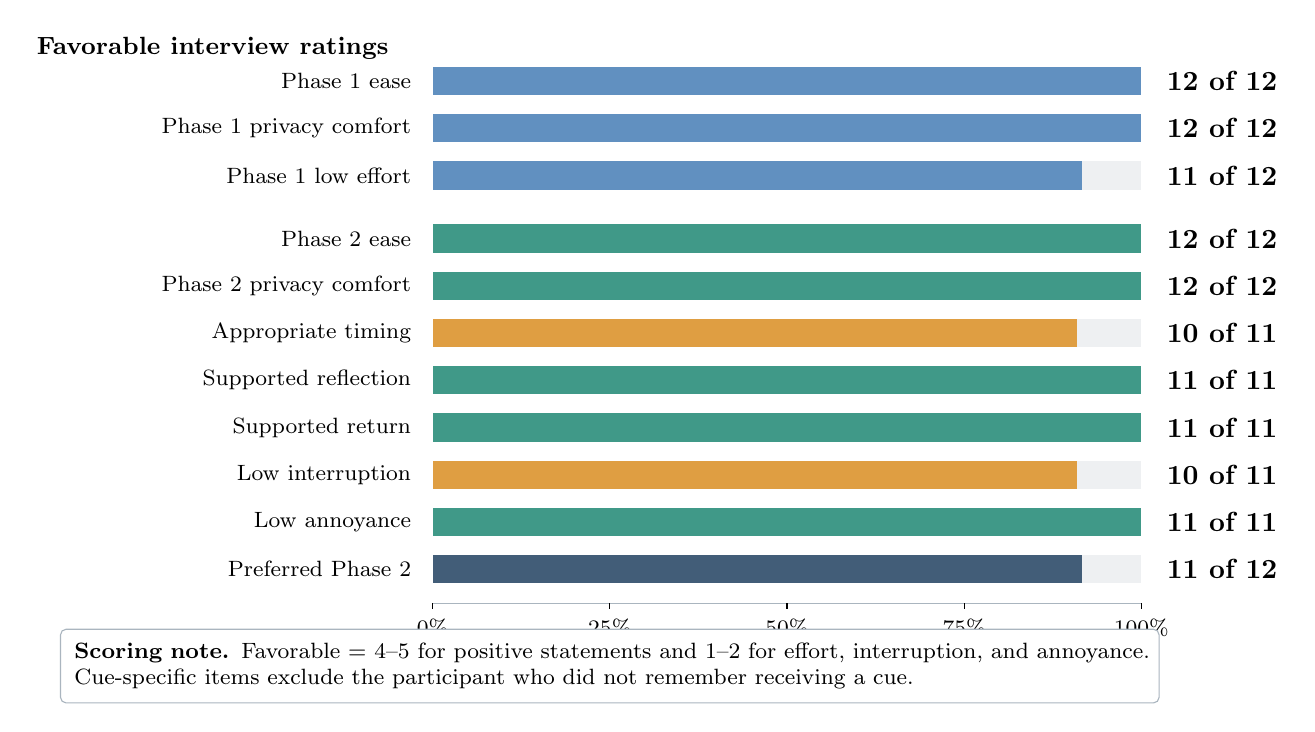
\begin{tikzpicture}[font=\fontsize{8.2}{9.5}\selectfont]
\node[anchor=west,font=\headingfont\bfseries\fontsize{9.5}{11}\selectfont] at (0,6.3) {Favorable interview ratings};
\node[anchor=east] at (5.0,5.88) {Phase 1 ease};
\node[anchor=east] at (5.0,5.28) {Phase 1 privacy comfort};
\node[anchor=east] at (5.0,4.68) {Phase 1 low effort};
\node[anchor=east] at (5.0,3.88) {Phase 2 ease};
\node[anchor=east] at (5.0,3.28) {Phase 2 privacy comfort};
\node[anchor=east] at (5.0,2.68) {Appropriate timing};
\node[anchor=east] at (5.0,2.08) {Supported reflection};
\node[anchor=east] at (5.0,1.48) {Supported return};
\node[anchor=east] at (5.0,.88) {Low interruption};
\node[anchor=east] at (5.0,.28) {Low annoyance};
\node[anchor=east] at (5.0,-.32) {Preferred Phase 2};
\foreach \y/\pct/\frac/\col in {
5.7/1.00/12 of 12/dsBlue,
5.1/1.00/12 of 12/dsBlue,
4.5/.917/11 of 12/dsBlue,
3.7/1.00/12 of 12/dsGreen,
3.1/1.00/12 of 12/dsGreen,
2.5/.909/10 of 11/dsGold,
1.9/1.00/11 of 11/dsGreen,
1.3/1.00/11 of 11/dsGreen,
.7/.909/10 of 11/dsGold,
.1/1.00/11 of 11/dsGreen,
-.5/.917/11 of 12/dsNavy}{
  \fill[dsRule!20] (5.15,\y) rectangle (14.15,\y+.36);
  \fill[\col!82] (5.15,\y) rectangle ({5.15+9*\pct},\y+.36);
  \node[anchor=west,font=\bfseries] at (14.35,\y+.18) {\frac};
}
\draw[draw=dsRule] (5.15,-.75)--(14.15,-.75);
\foreach \x/\lab in {5.15/0\%,7.4/25\%,9.65/50\%,11.9/75\%,14.15/100\%}{\draw (\x,-.75)--++(0,-.08);\node[below] at (\x,-.83){\lab};}
\node[rounded corners=2pt,draw=dsRule,fill=white,text width=13.6cm,align=left,inner sep=5pt] at (7.4,-1.55) {\textbf{Scoring note.} Favorable = 4--5 for positive statements and 1--2 for effort, interruption, and annoyance. Cue-specific items exclude the participant who did not remember receiving a cue.};
\end{tikzpicture}
}
\caption{Item-level favorable ratings from the completed post-study interviews. Fractions show favorable responses over valid responses; the bar length shows the same proportion.}
\label{fig:interview}
\end{figure}

Item medians were consistent with the favorable counts. Phase 1 ease had a median of 4.0; session clarity 4.5; outcome-question clarity and privacy comfort 5.0; and effort 2.0. Phase 2 ease and privacy comfort each had a median of 5.0, while effort had a median of 2.0. Among cue-specific items, timing had a median of 4.0; useful reconsideration, reflection, and return each had a median of 5.0; and interruption and annoyance each had a median of 2.0. Preference for Phase 2 had a median of 5.0.

Open responses clarify what the ratings meant to participants. Seven responses were grouped as goal reorientation and four as reflective awareness; the remaining participant did not remember cue exposure. Participants described pausing, comparing the current page with the declared task, closing unrelated tabs, or deliberately continuing when a detour still served the task. The physical cue was valued because it remained noticeable when the browser was not visually foregrounded, and several participants emphasized that it prompted a choice without blocking the page.

Critical responses were equally informative. Five participants described an occasional false cue, one described a cue as early, and one said timing was useful overall but not exact. Four did not remember a clearly false cue, and one did not remember exposure. Requested refinements included volume control, a temporary mute option, clearer connection and delivery feedback, longer card visibility, confirmation after choosing to continue, and showing the declared task context. These comments explain why low annoyance should not be treated as evidence of perfect timing.

\section{Discussion}

\subsection{From Website Control to Task-Relative Reflection}

DriftSense's main conceptual move is to place the task, rather than the website, at the center of digital-wellbeing support. This matters because mixed-use environments make domain labels brittle. The same approved hostname appeared across different task types in the dataset, and activity away from the approved set could be necessary background work. Requiring explicit task initiation and a later alignment answer makes the system legible: the user can see what was declared, what was measured, and what ultimately supplied the label.

The baseline progression supports this framing without proving semantics. Intended duration, task site, and task type alone showed limited discrimination, while aggregate activity substantially separated the two reported outcomes. Yet activity remained predictive rather than definitive. The model estimates whether a pattern resembles sessions later reported as moved away; it does not transform away time, idling, or tab switching into objective drift. This distinction is especially important when a cue is delivered during a live task.

\subsection{Why a Tangible Cue}

The ESP32 interface gives model timing a physical expression. Browser prompts compete with the same visual environment in which drift occurs and can be hidden behind windows or tabs. A brief audible cue and visible countdown can remain noticeable without covering content. Physical controls also make the interaction state explicit: start, finish, and final reflection are actions rather than inferred boundaries.

Participants' reports support this role. They commonly described the beep as brief, noticeable, and useful for returning to the task, including when the browser was not in front. Requests for volume control, muting, and connection feedback also show that a physical device introduces social and practical concerns. A sound suitable at a private desk may be unsuitable in a meeting or shared room. The next version should retain the physical cue while making volume and confirmation clearer.

\subsection{Interpreting the Two Evidence Streams}

The model and interview results are complementary but not interchangeable. The chronological holdout quantifies whether completed-session features distinguish later self-reports. It does not establish accuracy at minute 5 or minute 10. The interviews show how the deployed system was experienced by 12 participants. They do not independently verify each delivery time, nor do they prove that a cue caused a behavioral change. The paper's central claim is consequently an implemented and evaluated pathway from private sensing to tangible reflection, not a causal reduction in drift.

This separation strengthens the contribution. The completed data show that content-free session patterns carry useful retrospective signal; the deployed product shows that the decisions can drive a time-limited physical interaction; and the interviews identify both acceptance and concrete refinements. A future controlled study can build on these verified components without repeating the completed interviews.

\subsection{Relation to Prior Systems}

Like Purpose Mode, DriftSense preserves access and recognizes that browsing context can affect perceived goal alignment \citep{lee2025purpose}. Unlike Purpose Mode, it does not alter the content interface; it evaluates a participant-started task session and places reflection outside the page. Like \textit{one sec}, it uses a small interruption to create a decision point \citep{gruning2023onesec}. Its cue occurs during an unfolding task rather than before opening an application. Like StayFocused, it uses reflection instead of simple blocking \citep{li2024stayfocused}; however, its timing comes from content-free activity summaries and a duration-dependent policy rather than only attempted exit or completion.

The design also differs from tools that optimize screen-time reduction. DriftSense can treat a long session as aligned and a short session as drifted because the outcome refers to the participant's declared task. It can therefore support study, coding, research, communication, and planned leisure without ranking one category as better than another. Its deliberate limitation is that content-free sensing cannot explain why a pattern occurred; the participant's self-report remains necessary.

\subsection{Limitations}

The study has several limitations. First, the Phase 1 sample contains repeated sessions from 19 participants. The chronological holdout uses later records from known participants and cannot establish generalization to unseen users. Second, the operational model was trained and evaluated retrospectively on completed-session activity proportions. Although the 5/10-minute schedule is implemented, its early-window discrimination, calibration, and false-cue burden were not separately estimated from checkpoint outcomes.

Third, 31 sessions lacked a usable binary outcome and were excluded. Twenty numeric labels were reconciled against explicit answers. The rule was prespecified and transparent, but missingness and response error remain possible. Fourth, the interview sample is small, retrospective, and exposed to the phases in a fixed order. Recall, novelty, and social-desirability effects may influence the favorable ratings. One participant did not remember a cue, and the workbook is not a replacement for delivery logs.

Fifth, an audible cue can be inaccessible, unnoticed, or socially awkward. The prototype supports a short bounded beep, but participant requests show the need for configurable volume, silent modes, and clearer connection state. Finally, privacy minimization constrains model knowledge by design. Because DriftSense excludes page text and outside-set destination identity, it cannot determine semantic relevance. That limitation is also part of its contribution: the system asks for human interpretation rather than silently expanding surveillance.

\section{Conclusions}

DriftSense demonstrates a complete path from participant-declared browser tasks to model-timed tangible reflection. Phase 1 collected 665 sessions from 19 participants, preserved explicit self-report as the task-drift label, and produced a compact model with strong completed-session discrimination. Phase 2 converted that model into successive five- or ten-minute decisions and an ESP32 interface combining a countdown display, a brief beep, and three physical controls. Interviews with 12 participants indicated high usability and privacy comfort; the 11 who remembered the cue generally described it as useful and minimally annoying while also identifying occasional false or mistimed cues.

The resulting contribution is neither a website classifier nor a productivity score. It connects structured task context, content-free sensing, explicit outcome measurement, local prediction, and a physical point of reflection. Its next evaluation step is a controlled, window-level study of early prediction and behavioral effects, not broader or more invasive sensing.

\section{Implications for Theory, Application, or Policy}

DriftSense suggests that digital-wellbeing systems should represent alignment as a relationship between a declared task, an unfolding activity pattern, and a later human judgment. For theory, this separates behavioral evidence from its meaning and avoids equating duration with harm. For application, the results favor sparse, optional cues, participant-approved task sites, explicit session boundaries, and hardware controls that remain visible beyond the browser window. Configurable sound and clear delivery feedback should be treated as accessibility features, not optional polish. For research governance, data minimization should be specified by field: systems can retain timing and aggregate activity while excluding page content, destination histories, and key values. Evaluations should report completed-session accuracy, early-window accuracy, delivery reliability, and intervention effects separately so that an implemented cue is not mistaken for causal evidence.

\section*{Ethics Statement}

The session and interview findings are reported using anonymous participant identifiers and the consent procedure documented in the study materials. No participant names, page content, messages, source code, search queries, or destination sites outside the participant-approved task-site set are reported. Participation was voluntary, and the system supported local inspection, export, and deletion of records.

\section*{Data and Materials Availability}

The extension source, schemas, tests, analysis code, model documentation, and aggregate results are maintained with the project. Participant-level exports and interview records should be shared only when consent, institutional approval, and disclosure-risk review permit it. Any released aggregate or de-identified evidence should include field definitions, exclusion and reconciliation rules, model versions, and reproducible commands.

\printbibliography[title={References}]

\end{document}
